% vim:encoding=utf8 ft=tex sts=2 sw=2 et:

\documentclass{classrep}
\usepackage[utf8]{inputenc}

\usepackage[pdftex]{color,graphicx}
\DeclareGraphicsExtensions{.pdf,.png,.jpg}

\usepackage{float}

\usepackage{color}

\usepackage{listings}

\usepackage{color}

\usepackage[hyphens]{url}

\usepackage{hyperref}

\usepackage[polish]{babel}

\usepackage{enumitem}

\usepackage{indentfirst}
\usepackage[center,small,bf]{caption}
\hypersetup{colorlinks=false,pdfborder={0 0 0}}

\renewcommand{\labelitemi}{$\bullet$}
\renewcommand{\labelitemii}{$\cdot$}
\renewcommand{\labelitemiii}{$\diamond$}
\renewcommand{\labelitemiv}{$\ast$}
\definecolor{dkgreen}{rgb}{0,0.6,0}
\definecolor{gray}{rgb}{0.5,0.5,0.5}
\definecolor{mauve}{rgb}{0.58,0,0.82}
\lstset{ %
  language=Matlab,                % the language of the code
  basicstyle=\footnotesize,           % the size of the fonts that are used for the code
  numbers=left,                   % where to put the line-numbers
  numberstyle=\tiny\color{gray},  % the style that is used for the line-numbers
  stepnumber=2,                   % the step between two line-numbers. If it's 1, each line 
                                  % will be numbered
  numbersep=5pt,                  % how far the line-numbers are from the code
  backgroundcolor=\color{white},      % choose the background color. You must add \usepackage{color}
  showspaces=false,               % show spaces adding particular underscores
  showstringspaces=false,         % underline spaces within strings
  showtabs=false,                 % show tabs within strings adding particular underscores
  frame=single,                   % adds a~frame around the code
  rulecolor=\color{black},        % if not set, the frame-color may be changed on line-breaks within not-black text (e.g. commens (green here))
  tabsize=2,                      % sets default tabsize to 2 spaces
  captionpos=b,                   % sets the caption-position to bottom
  breaklines=true,                % sets automatic line breaking
  breakatwhitespace=false,        % sets if automatic breaks should only happen at whitespace
  title=\lstname,                   % show the filename of files included with \lstinputlisting;
                                  % also try caption instead of title
  keywordstyle=\color{blue},          % keyword style
  commentstyle=\color{dkgreen},       % comment style
  stringstyle=\color{mauve},         % string literal style
  escapeinside={\%*}{*)},            % if you want to add a~comment within your co
}
\hyphenation{Fibonacciego}

\studycycle{Informatyka, studia dzienne, mgr II st.}
\coursesemester{I}

\coursename{Metody obliczeniowe optymalizacji}
\courseyear{2011/2012}

\courseteacher{mgr inż. Łukasz Chomątek}
\coursegroup{czwartek, 16:00}

\author{
  \studentinfo{Paweł Musiał}{178726} \and
  \studentinfo{Łukasz Michalski}{178724}
}

\title{Zadanie 2: Optymalizacja kierunkowa}
\svnurl{https://serce.ics.p.lodz.pl/svn/labs/moo/lc_cz1600/lmpm}

\begin{document}
\maketitle

\addtocounter{footnote}{1}

\section{Cel}
Celem zadania było napisać program, który dla dowolnej funkcji dwóch zmiennych rozwiąże zadanie optymalizacji na odcinku. Optymalizacja kierunkowa musi być przeprowadzona z wykorzystaniem kryteriów:
\begin{itemize}
\item Armijo
\item Wolfa
\item Goldsteina
\end{itemize}
Przedstawiany jako rozwiązanie program powinien pozwolić wprowadzić funkcję oraz odcinek, w którym poszukiwane będzie rozwiązanie.

\section{Rozwiązanie zadania}
\subsection{Metoda najszybszego spadku}
Metoda najszybszego spadku jest iteracyjnym algorytmem wyszukiwania minimum zadanej funkcji celu $f$. Założenia dla metody są następujące:
\begin{itemize}
\item $f\in C^1$ (funkcja jest ciągła i różniczkowalna),
\item $f$ jest ściśle wypukła w badanej dziedzinie.
\end{itemize}
Poszukiwania te odbywają się na podstawie gradientu tej funkcji. Wiadomo, że gradient $\bigtriangledown f=[\frac{\partial f}{\partial x_{1}},...,\frac{\partial f}{\partial x_{n}}]^T$ ma ważną własność mówiącą że poruszając się z dowolnego punktu $x$ ,,w kierunku gradientu'' osiągamy (lokalnie) najszybszy przyrost funkcji. W myśl tej zasady, jeśli $\bigtriangledown f$ wyznacza najszybszy wzrost, to $-\bigtriangledown f$ wyznacza najszybszy spadek. Na tym spostrzeżeniu opiera się metoda najszybszego spadku, którą w skrócie można ja opisać następująco:
\begin{enumerate}
\item Znajdź najlepszy kierunek (kierunek najszybszego spadku),
\item Określ jak daleko chcesz ,,zrobić krok'' w tym kierunku,
\item Zrób krok i sprawdź warunek stopu.
\end{enumerate}

Problemem występującym przy zastosowaniu metody najszybszego spadku jest jej ,,spowolnienie'', gdy zbliża się do minimum (zmiany zmiennych zależna od wielkości gradientu, a gradient dąży do zera w otoczeniu punktu minimum). Alogrytm działania tej metody został przedstawiony na diagramie:
\begin{figure}[h!]
\centering
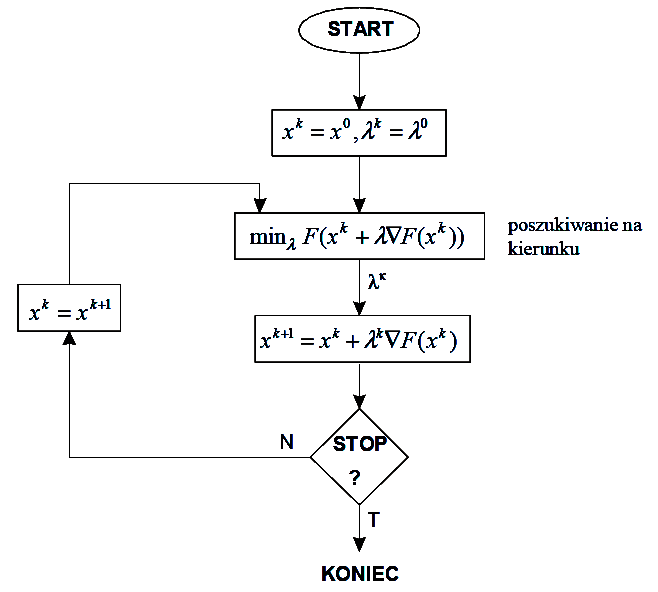
\includegraphics[width=10cm]{obrazy/metodaNS_algo} 
\caption{Schemat działania metody najszybszego spadku.\\*{\footnotesize Źródło: Wykład 4 Wojciecha Grega: Metody Optymalizacji}}
\label{fig:metodaNS_algo}
\end{figure}

Jak można zauważyć ważnym elementem tego algorytmu jest wybór odpowiedniej długość użytego kroku oraz kryterium stopu. Ma to bowiem wpływ na szybkość i stabilność działania oraz na osiągnięte wyniki. W tym zadaniu skupimy się na trzech kryteriach doboru optymalnego kroku:
\begin{itemize}
\item Armijo
\item Wolfa
\item Goldsteina
\end{itemize}

Na rysunku \ref{fig:metodaNS_przebieg} można zobaczyć przykład działania metody najszybszego spadku dla dwuwymiarowej funkcji celu. W każdym kroku, w zadanym kierunku wyszukiwana jest najmniejsza wartość funkcji celu.
\begin{figure}[h!]
\centering
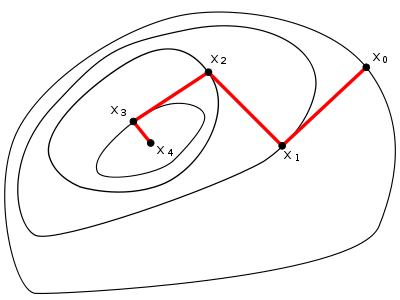
\includegraphics[width=6cm]{obrazy/metodaNS_przebieg} 
\caption{Przebieg działania metody najszybszego spadku. \\*{\footnotesize Źródło: \url{http://pl.wikipedia.org/wiki/Plik:Metoda_najszybszego_spadku.svg}}}
\label{fig:metodaNS_przebieg}
\end{figure}

\subsection{Kryterium Armijo}

\subsection{Kryterium Wolfa}

\subsection{Kryterium Goldsteina}


\section{Opis programu}
Program składa się z~implementacji trzech kryteriów.

\subsection{Metoda najszybszego spadku}
\begin{lstlisting}
\end{lstlisting}

\subsection{Kryterium Armijo}
\begin{lstlisting}
\end{lstlisting}

\subsection{Kryterium Wolfa}
\begin{lstlisting}
\end{lstlisting}

\subsection{Kryterium Goldsteina}
\begin{lstlisting}
\end{lstlisting}

\section{Wyniki}
	
\section{Wnioski}

\begin{thebibliography}{9}
\bibitem{1}
	Michał Lewandowski,  \emph{Metody optymalizacji - teoria i~wybrane algorytmy}.  2012.
\end{thebibliography}

\end{document}